\begin{figure}[H]
\centering
\resizebox{0.6\textwidth}{!}{
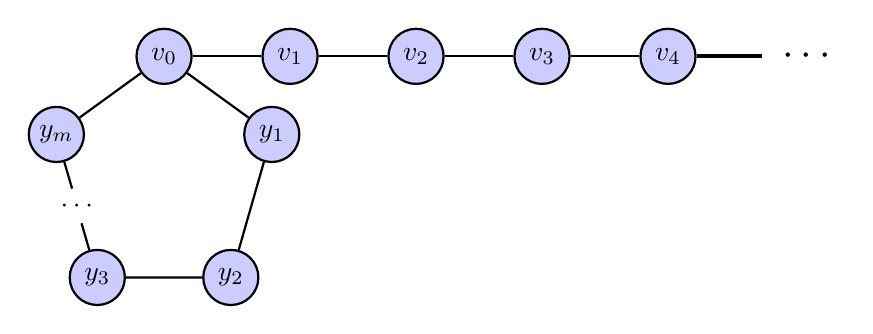
\begin{tikzpicture}[
  scale=0.8,
  vnode/.style={circle, fill=blue!20, draw=black, thick, inner sep=2pt, minimum size=7mm},
  edge/.style={thick, draw=black}
]

  % --- Vértice superior v_1 (origen del camino y del ciclo C^5) ---
  \node[vnode] (v1) at (0, 0) {$v_0$};

  % --- Vértices restantes del C^5 (disposición en pentágono regular simétrico abajo de v_1) ---
  \node[vnode] (y2) at (-1.71, -1.24) {$y_{m}$};
  \node[vnode] (y3) at ( 1.71, -1.24) {$y_1$};
  \node[vnode] (y4) at ( 1.06, -3.51) {$y_2$};
  \node[vnode] (y5) at (-1.06, -3.51) {$y_3$};

  % --- Aristas del ciclo C^5 con corte y puntos suspensivos horizontales ---
  \draw[edge] (v1) -- (y2);
  
  % Arista interrumpida entre y_n (y2) y y_4 (y5)
  \draw[edge] (y2) -- (-1.46, -2.1);
  \draw[edge] (-1.31, -2.65) -- (y5);
  \node[draw=none, fill=none] at (-1.385, -2.375) {$\cdots$};

  \draw[edge] (y5) -- (y4);
  \draw[edge] (y4) -- (y3);
  \draw[edge] (y3) -- (v1);

  % --- Camino horizontal superior (v_2 a v_5 y puntos suspensivos) ---
  \node[vnode] (v2) at (2.0, 0) {$v_1$};
  \node[vnode] (v3) at (4.0, 0) {$v_2$};
  \node[vnode] (v4) at (6.0, 0) {$v_3$};
  \node[vnode] (v5) at (8.0, 0) {$v_4$};

  \draw[edge] (v1) -- (v2);
  \draw[edge] (v2) -- (v3);
  \draw[edge] (v3) -- (v4);
  \draw[edge] (v4) -- (v5);
   
  % Continuación con puntos suspensivos
  \draw[edge, line width=1.5pt] (v5) -- (9.5, 0);
  \node[draw=none, fill=none, scale=1.5] at (10.2, 0) {$\cdots$};

\end{tikzpicture}}
\caption{El grafo $G_2$, con $m=n-1$}
\end{figure}
